% !TEX encoding = UTF-8 Unicode
% -*- coding: UTF-8; -*-
% vim: set fenc=utf-8

\section{Architektura}\label{sec:architektura}

Architektura určuje strukturu a části aplikace.
V této sekci vysvětlím jednotlivé části navržené architektury prototypu.

Navrženou architekturu rozdělím na tři část, klientskou, serverovou a databázovou část.
Jedná se o model klient-server (viz obrázek~\ref{fig:client_server}), protože jsou od sebe role klienta a serveru odděleny.
Komunikace mezi nimi probíhá pomocí předem definovaných aplikačních rozhraní postavených na protokolu \gls{HTTP} (více o rozhraní v sekcích~\ref{sec:restKomunikace} a~\ref{sec:komunikaceVeSkutečnémČase}).

\begin{figure}[ht!]
    \centering
    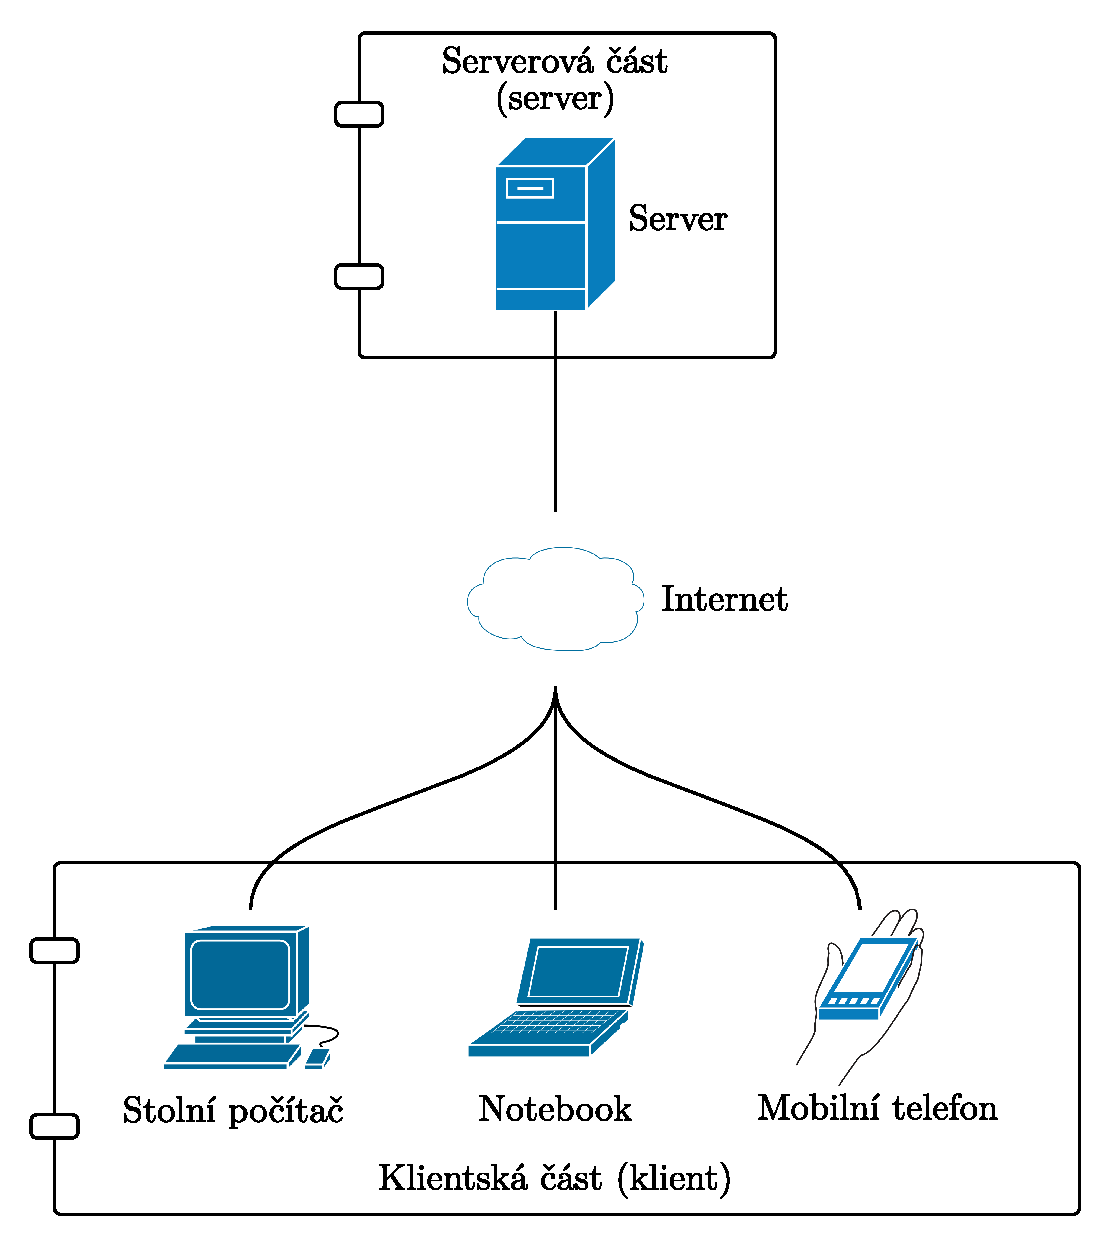
\includegraphics[width=0.8\textwidth]{partials/navrh/clientServer2.pdf}
    \caption{Diagram architektury aplikace (klient-server)}\label{fig:client_server}
\end{figure}

\subsection{Klientská část}\label{subsec:klientskáČást}

Jedná se o část aplikace, která běží v samotném prohlížeči uživatele.
Reaguje na uživatelský vstup, generuje uživatelské rozhraní podle stavu aplikace a pomocí protokolu \gls{HTTP} komunikuje se serverovou částí za účelem úpravy, či získání dat.

Klientská část je napsána v jazycích HTML5 a JavaScript, ale také využívá knihovny pro tvorbu uživatelského rozhraní ReactJS (více o technologií v sekci~\ref{sec:technologie}).

\subsection{Serverová část}\label{subsec:serverováČást}

Serverová část je centrem aplikace, její hlavní zodpovědností je poskytnutí autentizace a autorizace jednotlivých uživatelů.
Dále je tato část zodpovědná za zajištění konzistence dat v perzistentním (databázovém) uložišti a poskytuje rozhraní pro komunikaci s klientskou částí aplikace.

Serverová část využívá JavaScriptové běhové prostředí Node.js (více o prostření v sekci~\ref{subsec:nodejs}) a je navržena podle dvouvrstvé architektury.
Datová vrstva zajišťuje přístup k databázové části a za pomoci návrhového vzoru repositář (anglicky repository pattern) vystavuje rozhraní v rámci serverové části, které umožňuje přístup k datům.
Presenční vrstva zajišťuje komunikaci s klientskou části a validitu přijatých dat, volá jednotlivé funkce datové vrstvy za účelem získání, či uložení dat.

\subsection{Databázová čast}\label{subsec:databázováČast}

Tato poslední část aplikace je zodpovědná za poskytování rozhraní pro přístup a operace na perzistentním uložištěm.

Rozhodl jsem se pro použití \gls{SŘBD} MongoDB (více o databázích v sekci~\ref{subsec:databáze}).
MongoDB umožňuje rychlejší vývoj aplikací a pro problém editace textů se jako zástupce \gls{NoSQL} hodí lépe, než tradiční \gls{SQL} databáze.
U webové editoru textů lze očekávat stále rostoucí počet dokumentů a jejich úprav, což by mohl být pro \gls{SQL} databáze problém hlavně z pohledu budoucího škálování aplikace.

MongoDB poskytuje \gls{TCP/IP} rozhraní pro přístup a manipulaci s dokumenty, které následně využívá serverová část aplikace.

